% ============================================================================
% Self-contained proof:
%   Optimal pairwise einsum schedules attain the index-elimination
%   (treewidth) bound, in both time and space.
%
% This is a corrected and completed rewrite of Direction 2 (Section 3) of
% exploration.tex, intended for internal review before insertion into
% ustats_revision.tex.  A changelog relative to the exploration draft is in
% the final section.
%
% Cross-references to the main manuscript ("MS") are by name, not number:
%   - MS Proposition 1  = index-wise complexity bound  |A| n^{tw(G_A)+1}
%   - MS Definition (decomposition graph), (vertex elimination), (treewidth)
%   - MS Lemma (einsum-sequence <-> elimination)  = lem:einsum_graph_seq
% Update these to \ref's once merged into the revision.
% ============================================================================
\documentclass[11pt]{article}

\usepackage[a4paper, margin=1.1in]{geometry}
\usepackage[T1]{fontenc}
% \usepackage{lmodern}  % loaded by the project preamble; uncomment if standalone
\usepackage{amsmath,amssymb,amsthm,mathtools}
\usepackage{tikz}
\usetikzlibrary{arrows.meta, positioning, calc}

% ---- macros mirroring the main paper ----
\newcommand{\Einsum}{\textsc{Einsum}}
\newcommand{\calA}{\mathcal{A}}
\newcommand{\calB}{\mathcal{B}}
\newcommand{\calS}{\mathcal{S}}
\newcommand{\calT}{\mathcal{T}}
\newcommand{\tw}{\mathrm{tw}}
\newcommand{\treewidthp}[1]{\tw(#1)}
\newcommand{\takesetp}[1]{\mathrm{Set}(#1)}
\newcommand{\degp}[2]{\deg_{#2}(#1)}
\newcommand{\eliminatevg}[2]{\mathsf{Elim}_{#1}(#2)}
\newcommand{\graphform}[1]{G_{#1}}
\newcommand{\wid}{\mathrm{w}}
\newcommand{\Time}{\mathrm{Time}}
\newcommand{\Aux}{\mathrm{Aux}}
\newcommand{\opteinsum}{\texttt{opt\_einsum}}
\newcommand{\torcheinsum}{\texttt{torch.einsum}}

\theoremstyle{plain}
\newtheorem{theorem}{Theorem}
\newtheorem{lemma}{Lemma}
\newtheorem{proposition}{Proposition}
\newtheorem{corollary}{Corollary}
\newtheorem{fact}{Fact}
\theoremstyle{definition}
\newtheorem{definition}{Definition}
\newtheorem{assumption}{Assumption}
\theoremstyle{remark}
\newtheorem{remark}{Remark}

\title{Optimal pairwise \Einsum{} schedules attain the\\
index-elimination bound, in time and space}
\author{}
\date{}

\begin{document}
\maketitle

\begin{abstract}
\noindent
We formalize the pairwise (binary) and unary primitives used by
\torcheinsum{} and \opteinsum{} to evaluate an \Einsum{} expression, and
prove that the optimal time complexity over all pairwise schedules equals,
up to factors not depending on the sample size $n$, the index-wise
elimination bound $n^{\treewidthp{\graphform{\calA}}+1}$ of Proposition~1 of the
main manuscript.  Moreover, an optimal pairwise schedule can be chosen so
that its peak working memory beyond the input tensors is also
$O(n^{\treewidthp{\graphform{\calA}}+1})$.  The unary primitive is necessary: with
binary primitives alone the equivalence fails, as witnessed by the
distance-covariance signature $\calA=((1,2),(3,4))$.
\end{abstract}

% ============================================================================
\section{Setting and recalled facts}
\label{sec:setup}
% ============================================================================

Throughout, $\calA = (A_1,\dots,A_K)$ is an \Einsum{} notation with empty
output ($B=\emptyset$) and index set $[m]$; the corresponding tensor tuple
is $\calT = (T_1,\dots,T_K)$, where $T_k$ has one mode per entry of $A_k$
and every mode has size $n$.  For a tuple $A$ we write $\takesetp{A}$ for
its set of entries.  The goal is to compute the scalar
\begin{align*}
   \Einsum(\calT,\calA)
   \;=\;
   \sum_{\alpha \in [n]^m}\; \prod_{k=1}^{K} T_k\bigl(\alpha[A_k]\bigr).
\end{align*}

We make the following standing assumptions.

\begin{assumption}
\label{ass:standing}
(i)~The entries of each $A_k$ are pairwise distinct; (ii)~every index
$i \in [m]$ occurs in at least one $A_k$; (iii)~for the space statements
only, $m \le n$.
\end{assumption}

Assumption~(i) holds for every tensorized multiplicative-decomposable
kernel in the main manuscript, and (iii) always holds in the
$U$-statistic setting, where $m$ is the order of the statistic and $n$ the
sample size.  We henceforth identify each signature with its index
\emph{set}; under (i) no information is lost.

\paragraph{Decomposition graph and elimination.}
Recall from the main manuscript (``MS'' hereafter) that the
\emph{decomposition graph} $\graphform{\calA}$ has vertex set $[m]$ and an
edge $\{i,j\}$ if and only if $i$ and $j$ co-occur in some $A_k$.
\emph{Vertex elimination} $\eliminatevg{v}{G}$ deletes $v$ and connects
$N_G(v)$ into a clique.  Given a permutation $\sigma$ of $[m]$, set
$G^\sigma_0 \coloneqq \graphform{\calA}$ and
$G^\sigma_i \coloneqq \eliminatevg{\sigma[i]}{G^\sigma_{i-1}}$.  The
\emph{elimination width} of $\sigma$ is
\begin{align*}
   \wid(\sigma) \;\coloneqq\; \max_{i \in [m]}\;
   \degp{\sigma[i]}{G^\sigma_{i-1}},
\end{align*}
and, as in MS Definition~(treewidth via elimination),
$\treewidthp{\graphform{\calA}} = \min_\sigma \wid(\sigma)$.

We will use two facts.  The first is proved in MS; the second is a
standard property of vertex elimination which we prove for completeness,
as it does the bookkeeping for fill-in edges and for ties in our lower
bound.

\begin{fact}[MS, \Einsum{}-sequence $\leftrightarrow$ elimination]
\label{fact:ms}
Let $\calA^\sigma_0,\dots,\calA^\sigma_m$ be the \Einsum{} notation
sequence of $\calA$ under $\sigma$ (MS Definition: at step $i$, all tuples
containing $\sigma[i]$ are removed and the single tuple
$s_{\sigma[i]} \coloneqq \bigcup_{A \ni \sigma[i]} \takesetp{A} \setminus
\{\sigma[i]\}$ is inserted if nonempty).  Then
$\graphform{\calA^\sigma_i} = G^\sigma_i$ for every $i$.  In particular,
for every tuple $A \in \calA^\sigma_{i-1}$ with $\sigma[i] \in A$,
\begin{align*}
   \takesetp{A} \;\subseteq\; \{\sigma[i]\} \cup
   N_{G^\sigma_{i-1}}(\sigma[i]).
\end{align*}
\end{fact}

\begin{fact}[Elimination of a set; order independence]
\label{fact:set-elim}
Let $G$ be a graph and $S \subseteq V(G)$.  Eliminate the vertices of $S$
one by one, in any order.  The resulting graph on $V(G)\setminus S$ does
not depend on the order, and two vertices $u,v \notin S$ are adjacent in
it if and only if $G$ contains a $u$--$v$ path all of whose internal
vertices lie in $S$ (a direct edge counting as such a path).  We denote
this graph by $G \ominus S$.
\end{fact}

\begin{proof}
Induction on $|S|$.  For $S=\emptyset$ both claims are trivial.  Let
$s \in S$ be eliminated first and $G' \coloneqq \eliminatevg{s}{G}$, so that
$u,v$ are adjacent in $G'$ iff they are adjacent in $G$ or both are
$G$-neighbors of $s$; equivalently, iff $G$ has a $u$--$v$ path internal
to $\{s\}$.  By the inductive hypothesis applied to $(G', S\setminus\{s\})$,
the final graph has $u \sim v$ iff $G'$ contains a $u$--$v$ path internal
to $S \setminus \{s\}$.  Expanding each $G'$-edge of such a path into a
$G$-edge or a length-two $G$-path through $s$ yields a $u$--$v$ path in
$G$ internal to $S$; conversely, given a $u$--$v$ path in $G$ internal to
$S$, taken simple so that it visits $s$ at most once, replacing the
(possible) visit $x$--$s$--$y$ by the $G'$-edge $x$--$y$ yields a
$u$--$v$ path in $G'$ internal to $S\setminus\{s\}$.  Hence the
characterization holds and is order independent.
\end{proof}

Note that with $E_{i-1} \coloneqq \{\sigma[1],\dots,\sigma[i-1]\}$ we have
$G^\sigma_{i-1} = \graphform{\calA} \ominus E_{i-1}$, so
Fact~\ref{fact:set-elim} gives the explicit description
\begin{equation}
\label{eq:nbhd}
   N_{G^\sigma_{i-1}}(c)
   \;=\;
   \bigl\{\, u \notin E_{i-1}\cup\{c\} :\,
   \graphform{\calA} \text{ has a } c\text{--}u \text{ path internal to }
   E_{i-1} \,\bigr\},
   \qquad c \coloneqq \sigma[i].
\end{equation}

% ============================================================================
\section{The pairwise computation model}
\label{sec:model}
% ============================================================================

We now formalize the operations from which \torcheinsum{} and
\opteinsum{} build their contraction paths: binary contractions of two
tensors (including broadcasts and outer products as degenerate cases) and
unary reductions of a single tensor.

\begin{definition}[Primitives]
\label{def:primitives}
A \emph{primitive} acts on the current tensor list $\calS$ with signature
list $\calB$, consumes its operand(s), and appends one new tensor.
\begin{itemize}
\item[\textbf{(P1)}] \textbf{Binary contraction.}  Choose distinct
$T_a, T_b \in \calS$ with signatures $B_a, B_b$, and a (possibly empty)
set $C \subseteq \takesetp{B_a} \cup \takesetp{B_b}$ of \emph{eliminated}
indices such that no index of $C$ occurs in any signature of
$\calB$ other than $B_a, B_b$.  The output is
\begin{align*}
   T_c(\gamma) \;=\; \sum_{\alpha \in [n]^{C}}\,
   T_a\bigl((\gamma,\alpha)[B_a]\bigr)\cdot
   T_b\bigl((\gamma,\alpha)[B_b]\bigr),
   \qquad
   \takesetp{B_c} = \bigl(\takesetp{B_a}\cup\takesetp{B_b}\bigr)\setminus C .
\end{align*}
Its \emph{time cost} is $n^{|\takesetp{B_a}\,\cup\,\takesetp{B_b}|}$ and its
output occupies $n^{|B_c|}$ entries.
\item[\textbf{(P2)}] \textbf{Unary reduction.}  Choose $T_a \in \calS$
with signature $B_a$ and a nonempty $C \subseteq \takesetp{B_a}$ such that
no index of $C$ occurs in any other signature of $\calB$.  The output is
$T_c(\gamma) = \sum_{\alpha\in[n]^C} T_a\bigl((\gamma,\alpha)[B_a]\bigr)$
with $\takesetp{B_c} = \takesetp{B_a}\setminus C$, time cost
$n^{|B_a|}$, and output size $n^{|B_c|}$.
\end{itemize}
\end{definition}

\begin{remark}[Relation to the draft's three primitives, and to practice]
\label{rem:naming}
The earlier exploration draft listed three primitives.  Its binary
broadcast multiplication is the special case $C=\emptyset$ of (P1) with
$\takesetp{B_a}\cap\takesetp{B_b}\neq\emptyset$ (shared indices aligned but
not summed, because they still occur elsewhere); the outer product is the
case $C=\emptyset$ with disjoint signatures; its unary partial trace is
(P2) above.  We also allow $C \not\subseteq
\takesetp{B_a}\cap\takesetp{B_b}$ in (P1), i.e.\ a binary call may sum an
index appearing in only one operand --- exactly as a single
\texttt{einsum("ij,kl->ik",\,A,\,B)} call does.  This makes the model at
least as strong as the implemented one, which only strengthens the lower
bound below; the upper-bound construction uses only $C=\emptyset$ or
$C \subseteq \takesetp{B_a}\cap\takesetp{B_b}$, so it remains valid in the
narrower model as well.
\end{remark}

\begin{definition}[Schedule; time and space]
\label{def:schedule}
A \emph{pairwise schedule} $\Sigma$ for $(\calT,\calA)$ is a finite
sequence of primitives that, applied starting from $(\calT,\calA)$,
terminates with a list containing a single scalar.  Its \emph{time cost}
$\Time(\Sigma)$ is the sum of the time costs of its primitives.  For
space, we adopt the convention that every tensor (input or intermediate)
is freed at the end of the primitive in which it is last used; the
\emph{auxiliary space} $\Aux(\Sigma)$ is the maximum, over the execution,
of the total number of entries of all currently allocated
\emph{non-input} tensors.  (The inputs occupy $\sum_k n^{|A_k|}$ further
entries until freed; we account for them separately.)
\end{definition}

\begin{definition}[Induced elimination orderings]
\label{def:induced}
Indices disappear from the signature list only through the sets $C$ of
(P1)/(P2) primitives, and since the list ends at a scalar, every index of
$[m]$ disappears exactly once.  A permutation $\sigma$ of $[m]$ is
\emph{induced by} $\Sigma$ if it is consistent with the order of
disappearance; indices eliminated by the same primitive may be ordered
arbitrarily among themselves.  We write $\sigma \vartriangleleft \Sigma$.
\end{definition}

% ============================================================================
\section{Lower bound: every schedule pays its elimination width}
\label{sec:lower}
% ============================================================================

The lower bound rests on one invariant.  For a schedule $\Sigma$ and
$t \ge 0$, let $D_t \subseteq [m]$ denote the set of indices eliminated by
the first $t$ primitives, and let
$H_t \coloneqq \graphform{\calA} \ominus D_t$
(well defined by Fact~\ref{fact:set-elim}).  Call two surviving indices
\emph{co-resident at time $t$} if they occur together in some signature of
the list after $t$ primitives.

\begin{lemma}[Co-residence invariant]
\label{lem:invariant}
For every schedule $\Sigma$ and every $t \ge 0$: every edge of $H_t$ joins
two indices that are co-resident at time $t$.
\end{lemma}

\begin{proof}
Induction on $t$.  At $t=0$, $H_0 = \graphform{\calA}$ and its edges are,
by definition of the decomposition graph, precisely the co-occurrences
within input signatures.

For the step, suppose the claim holds at time $t$ and let the
$(t{+}1)$-st primitive have operand signature(s) $B_a$ (and $B_b$ if
binary) and elimination set $C$ (possibly empty), so
$D_{t+1} = D_t \cup C$.  Write $\mathcal{O} \coloneqq \takesetp{B_a}$ or
$\takesetp{B_a}\cup\takesetp{B_b}$ for the union of operand indices, and
recall the output signature is $\mathcal{O}\setminus C$.  We use
repeatedly the legality condition of Definition~\ref{def:primitives}:
\emph{every} signature of the time-$t$ list containing an index of $C$ is
an operand signature.

Let $\{u,v\}$ be an edge of $H_{t+1}$; by Fact~\ref{fact:set-elim} there
is a $u$--$v$ path in $\graphform{\calA}$ internal to $D_t \cup C$.
Contracting its maximal runs of $D_t$-vertices (each such run joins, by
Fact~\ref{fact:set-elim} applied to $D_t$, two vertices adjacent in
$H_t$), we obtain a $u$--$v$ path
\begin{align*}
   u \;-\; z_1 \;-\; z_2 \;-\;\cdots\;-\; z_q \;-\; v ,
   \qquad z_1,\dots,z_q \in C,\; q\ge 0,
\end{align*}
in $H_t$.  We distinguish two cases.

\emph{Case $q = 0$.}  Then $\{u,v\}$ is an edge of $H_t$, hence by the
inductive hypothesis $u,v$ are co-resident at time $t$, in some tensor
$T$.  If $T$ is not an operand it survives untouched and $u,v$ remain
co-resident.  If $T$ is an operand then $u,v \in \mathcal{O}$, and since
$u,v \notin C$ (they survive to time $t+1$) they lie in the output
signature $\mathcal{O}\setminus C$ and are co-resident in the output.

\emph{Case $q \ge 1$.}  Each consecutive pair on the path is an
$H_t$-edge, hence co-resident at time $t$ by the inductive hypothesis.
The witness tensor of $\{u,z_1\}$ contains $z_1 \in C$, hence is an
operand; therefore $u \in \mathcal{O}$.  Symmetrically
$v \in \mathcal{O}$.  As $u,v \notin C$, both lie in the output signature
and are co-resident at time $t+1$.
\end{proof}

\begin{lemma}[Per-index cost]
\label{lem:per-index}
Let $\Sigma$ be a schedule and $\sigma \vartriangleleft \Sigma$.  Fix
$i \in [m]$ and let the primitive eliminating $c \coloneqq \sigma[i]$ have
operand index union $\mathcal{O}$ as above.  Then
\begin{align*}
   \mathcal{O} \;\supseteq\; \{c\} \cup N_{G^\sigma_{i-1}}(c),
   \qquad\text{hence the primitive's time cost is at least }
   n^{\,1 + \degp{c}{G^\sigma_{i-1}}} .
\end{align*}
\end{lemma}

\begin{proof}
Let the primitive be the $(t{+}1)$-st, with elimination set $C \ni c$.
Since $\sigma$ is consistent with disappearance order,
$E_{i-1} = \{\sigma[1],\dots,\sigma[i-1]\} = D_t \cup C_{<}$, where
$C_{<} \subseteq C$ collects the indices of $C$ placed before $c$ by the
tie-break.

Let $u \in N_{G^\sigma_{i-1}}(c)$.  By \eqref{eq:nbhd} there is a
$c$--$u$ path in $\graphform{\calA}$ internal to $E_{i-1} \subseteq
D_t \cup C$.  Contracting its runs of $D_t$-vertices as in the previous
proof yields a path
$c - y_1 - \cdots - y_s - u$ in $H_t$ with $y_1,\dots,y_s \in C_{<}
\subseteq C$ and $s \ge 0$.  Every consecutive pair on this path is an
$H_t$-edge, hence co-resident at time $t$ (Lemma~\ref{lem:invariant}).
The witness tensor of the first edge contains $c \in C$, hence is an
operand, so its other endpoint ($y_1$, or $u$ if $s=0$) lies in
$\mathcal{O}$.  Proceeding along the path, the witness of $\{y_j,
y_{j+1}\}$ contains $y_j \in C$, hence is an operand, so $y_{j+1} \in
\mathcal{O}$; finally the witness of $\{y_s, u\}$ contains $y_s \in C$,
so $u \in \mathcal{O}$.  Also $c \in \mathcal{O}$ trivially.  Since the
primitive's time cost is $n^{|\mathcal{O}|}$ in either case of
Definition~\ref{def:primitives}, the bound follows.
\end{proof}

Note that Lemma~\ref{lem:per-index} holds for \emph{every} tie-break: the
argument used only $C_{<} \subseteq C$.  Taking the most expensive index
of each primitive and minimizing over orderings gives:

\begin{corollary}[Time lower bound]
\label{cor:lower}
For every pairwise schedule $\Sigma$ and every
$\sigma \vartriangleleft \Sigma$,
\begin{align*}
   \Time(\Sigma) \;\ge\; n^{\,1+\wid(\sigma)}
   \;\ge\; n^{\,\treewidthp{\graphform{\calA}}+1} .
\end{align*}
\end{corollary}

\begin{proof}
For each $i$, the primitive eliminating $\sigma[i]$ costs at least
$n^{1+\deg_{G^\sigma_{i-1}}(\sigma[i])}$ by Lemma~\ref{lem:per-index}, and
$\Time(\Sigma)$ is at least the cost of its most expensive primitive.
Hence $\Time(\Sigma) \ge n^{1+\wid(\sigma)} \ge
n^{1+\min_{\sigma'}\wid(\sigma')} = n^{\treewidthp{\graphform{\calA}}+1}$.
\end{proof}

% ============================================================================
\section{Upper bound: simulating an elimination ordering}
\label{sec:upper}
% ============================================================================

\begin{lemma}[Elimination $\Rightarrow$ schedule]
\label{lem:elim-to-schedule}
For every permutation $\sigma$ of $[m]$ there is a pairwise schedule
$\Sigma_\sigma$ with $\sigma \vartriangleleft \Sigma_\sigma$ such that
\begin{align*}
   \Time(\Sigma_\sigma) \;\le\; (K+m)\, n^{\,1+\wid(\sigma)} + K,
   \qquad
   \Aux(\Sigma_\sigma) \;\le\; 2\,n^{\,1+\wid(\sigma)} + m\, n^{\,\wid(\sigma)} .
\end{align*}
Under Assumption~\ref{ass:standing}(iii) ($m\le n$) the space bound is
$\le 3\,n^{\,1+\wid(\sigma)}$.  Moreover $\Sigma_\sigma$ only uses (P1)
with $C = \emptyset$ and (P2) with $|C|=1$, so it is implementable with
broadcast multiplications and single-index unary reductions alone.
\end{lemma}

\begin{proof}
\emph{Construction.}  We process $i = 1,\dots,m$ and maintain the
invariant
\begin{itemize}
\item[$(\star)$] after step $i$, the current signature list consists of
the tuples of $\calA^\sigma_i$ (as index sets), plus possibly some
scalars (empty signatures).
\end{itemize}
At the start, $(\star)$ holds with $\calA^\sigma_0 = \calA$.  At step
$i$, let $\calS_i^{\mathrm{in}} = (T_{(1)},\dots,T_{(r)})$ be the current
tensors whose signature contains $\sigma[i]$; by $(\star)$ and
Assumption~\ref{ass:standing}(ii) applied along the recursion,
$r \ge 1$.
\begin{itemize}
\item If $r=1$: apply (P2) to $T_{(1)}$ with $C=\{\sigma[i]\}$.  This is
legal because $\sigma[i]$ occurs in no other signature.
\item If $r\ge 2$: form the rolling products
$W_1 \coloneqq T_{(1)}$ and, for $j = 2,\dots,r$,
$W_j \coloneqq$ (P1) applied to $W_{j-1}$ and $T_{(j)}$ with
$C=\emptyset$; then apply (P2) to $W_r$ with $C=\{\sigma[i]\}$, which is
legal because every tensor whose signature contained $\sigma[i]$ has been
consumed into $W_r$.
\end{itemize}
In both cases the step consumes exactly the tuples of
$\calA^\sigma_{i-1}$ containing $\sigma[i]$ and produces one tensor with
signature $s_{\sigma[i]} = \bigcup_{j\le r}\takesetp{B_{(j)}} \setminus
\{\sigma[i]\}$ --- precisely the replacement defining
$\calA^\sigma_{i}$ --- or a scalar if $s_{\sigma[i]} = \emptyset$.  Hence
$(\star)$ is maintained.  After step $m$ the list contains only scalars
(at least one, at most $K$); multiply them pairwise by (P1) with
$C=\emptyset$ until a single scalar remains.  No index disappears except
$\sigma[i]$ at step $i$, so $\sigma \vartriangleleft \Sigma_\sigma$
exactly.

\emph{Time.}  Fix $i$ and abbreviate
$d_i \coloneqq \degp{\sigma[i]}{G^\sigma_{i-1}}$.  By $(\star)$, every
$B_{(j)}$ is a tuple of $\calA^\sigma_{i-1}$ containing $\sigma[i]$, so
Fact~\ref{fact:ms} gives $\takesetp{B_{(j)}} \subseteq \{\sigma[i]\}\cup
N_{G^\sigma_{i-1}}(\sigma[i])$, and therefore every rolling signature
satisfies
\begin{align*}
   \takesetp{W_j} \;=\; \bigcup_{l\le j} \takesetp{B_{(l)}}
   \;\subseteq\; \{\sigma[i]\}\cup N_{G^\sigma_{i-1}}(\sigma[i]),
   \qquad |\takesetp{W_j}| \le d_i + 1 .
\end{align*}
Hence each of the $r_i$ primitives of step $i$ ($r_i-1$ broadcasts and
one reduction, or a single reduction if $r_i=1$) costs at most
$n^{1+d_i} \le n^{1+\wid(\sigma)}$.  Each step consumes $r_i$ tensors and
produces one, so $\sum_i (r_i - 1) = K - c$, where $c\ge1$ is the number
of scalars left after step $m$; thus $\sum_i r_i = K - c + m \le K + m$.
The final $c-1$ scalar multiplications cost $1$ each.  Summing,
$\Time(\Sigma_\sigma) \le (K+m)\,n^{1+\wid(\sigma)} + K$.

\emph{Space.}  At any moment during step $i$, the allocated non-input
tensors are: (a)~at most two rolling tensors ($W_{j-1}$ while $W_j$ is
being written), each of at most $n^{1+d_i} \le n^{1+\wid(\sigma)}$
entries; and (b)~the outputs of completed steps $j<i$ not yet consumed.
Each output of step $j$ has signature $s_{\sigma[j]}$ of size
$\degp{\sigma[j]}{G^\sigma_{j-1}} \le \wid(\sigma)$, hence at most
$n^{\wid(\sigma)}$ entries, and there are fewer than $m$ of them.  Inputs
are freed when consumed.  Therefore
$\Aux(\Sigma_\sigma) \le 2 n^{1+\wid(\sigma)} + m\, n^{\wid(\sigma)}$,
which is at most $3 n^{1+\wid(\sigma)}$ when $m\le n$.
\end{proof}

\begin{remark}
\label{rem:early-contraction}
Unlike the exploration draft, the construction never sums out an
auxiliary index $j\neq\sigma[i]$ ``opportunistically'' during step $i$,
even when $j$ happens to occur only inside $\calS_i^{\mathrm{in}}$:
doing so would make $\sigma \vartriangleleft \Sigma_\sigma$ fail whenever
$j$ is not adjacent to $\sigma[i]$ in $\sigma$.  Such an index is instead
eliminated at its own step via the $r=1$ branch, at cost
$n^{1+d} \le n^{1+\wid(\sigma)}$.  The opportunistic variant remains a
valid schedule with the same bounds; only the induced-ordering claim
requires the discipline above.
\end{remark}

% ============================================================================
\section{Main result and consequences}
\label{sec:main}
% ============================================================================

\begin{theorem}[Pairwise $=$ index-wise, at optimality]
\label{thm:main}
Let $C^\ast_{\mathrm{pair}}(\calA)$ be the minimum of $\Time(\Sigma)$
over all pairwise schedules.  Then
\begin{align*}
   n^{\,\treewidthp{\graphform{\calA}}+1}
   \;\le\;
   C^\ast_{\mathrm{pair}}(\calA)
   \;\le\;
   (K+m)\, n^{\,\treewidthp{\graphform{\calA}}+1} + K .
\end{align*}
Consequently, for fixed \Einsum{} structure $\calA$ and $n\to\infty$,
$C^\ast_{\mathrm{pair}}(\calA) = \Theta\bigl(n^{\treewidthp{\graphform{\calA}}+1}\bigr)$,
matching the optimal index-wise complexity of MS Proposition~1 up to
factors depending only on $\calA$.  Moreover, a schedule attaining the
upper bound can be chosen with auxiliary space
$O\bigl(n^{\treewidthp{\graphform{\calA}}+1}\bigr)$ beyond the
$\sum_{k} n^{|A_k|}$ entries of the inputs, provided $m\le n$.
\end{theorem}

\begin{proof}
The lower bound is Corollary~\ref{cor:lower}.  For the upper bound and
the space claim, apply Lemma~\ref{lem:elim-to-schedule} to a permutation
$\sigma^\ast$ with $\wid(\sigma^\ast) = \treewidthp{\graphform{\calA}}$, which
exists by the elimination characterization of treewidth.
\end{proof}

\begin{remark}[On the prefactor]
\label{rem:prefactor}
The lower bound carries no factor $K=|\calA|$: a single (P1) call may
eliminate several indices at once, and the trivial input-reading bound
only gives $\Time(\Sigma) \ge \max_k n^{|A_k|}$, which is dominated by
$n^{\tw+1}$ since each $\takesetp{A_k}$ is a clique of
$\graphform{\calA}$ and hence $|A_k| \le \treewidthp{\graphform{\calA}}+1$.  The
statement ``$C^\ast_{\mathrm{pair}} \asymp |\calA|\,
n^{\treewidthp{\graphform{\calA}}+1}$'' of the exploration draft is therefore to
be read, like MS Proposition~1 itself, in the regime of fixed kernel
structure and growing $n$; the theorem above makes the constants
explicit.  Finding $\sigma^\ast$ remains NP-hard in general
(Arnborg--Corneil--Proskurowski), exactly as discussed in MS
Remark~(ordering in practice); the theorem concerns the complexity of
\emph{executing} an optimal schedule, not of \emph{finding} one.
\end{remark}

\begin{corollary}[Space complexity of the $V$- and $U$-statistic
algorithms]
\label{cor:space}
Under the conditions of MS Proposition~1, the \Einsum{} evaluation of a
$V$-statistic with signature $\calA$ can be executed with peak working
memory $O\bigl(n^{\treewidthp{\graphform{\calA}}+1}\bigr)$ beyond the input
tensorization.  Consequently, the $U$-statistic algorithm (MS
Algorithm~4), which evaluates one restricted $V$-statistic per partition
$\pi \in \Pi^{\calA}_m$ and accumulates the scalar results with their
M\"obius weights, can be executed with peak working memory
\begin{align*}
   O\bigl(n^{\,M+1}\bigr) + \textstyle\sum_{k} n^{|A_k|},
   \qquad
   M \coloneqq \max_{\pi \in \Pi^{\calA}_m} \treewidthp{\graphform{\calA}/\pi},
\end{align*}
by executing the partitions sequentially and freeing all intermediates of
one partition before starting the next.
\end{corollary}

\begin{proof}
Apply Theorem~\ref{thm:main} to each quotient signature; its index count
is at most $m \le n$, so the space statement applies.  The quotients
share the (sparsified) tensorization, which is allocated once; across
partitions only the running scalar accumulator persists.
\end{proof}

% ----------------------------------------------------------------------------
\subsection{Necessity of the unary primitive}
% ----------------------------------------------------------------------------

\begin{remark}[Binary-only schedules are not enough]
\label{rem:dcov}
Consider the dCov-type signature $\calA = ((1,2),(3,4))$, for which
$\graphform{\calA}$ is two disjoint edges and
$\treewidthp{\graphform{\calA}}+1 = 2$.  A schedule may reduce each $T_k$ to a
scalar by (P2) at cost $n^2$ and multiply the scalars, achieving the bound
of Theorem~\ref{thm:main} with $O(1)$ auxiliary space.  If (P2) is
forbidden, the first primitive must be a binary one, and the only two
tensors available are $T_1$ and $T_2$; whatever the choice of $C$, its
time cost is $n^{|\takesetp{B_1}\cup\takesetp{B_2}|} = n^4$.  Hence every
unary-free schedule has $\Time \ge n^4$, and the equivalence of
Theorem~\ref{thm:main} fails.  If, in addition, binary contractions may
only sum \emph{shared} indices ($C \subseteq
\takesetp{B_a}\cap\takesetp{B_b}$, as in \texttt{tensordot}-backed pairwise
kernels), the forced first step is the outer product $C=\emptyset$, which
also \emph{materializes} an order-$4$ intermediate: peak space
$\Theta(n^4)$ as well.  This is the implementation-level reason that
\torcheinsum{}/\opteinsum{} must dispatch single-tensor reductions
through a genuine unary path for the theorem to apply to them, and it
reproduces the empirical $n^4$ blow-up recorded in the commented-out
Table~6 of the main manuscript.
\end{remark}

\begin{figure}[ht]
\centering
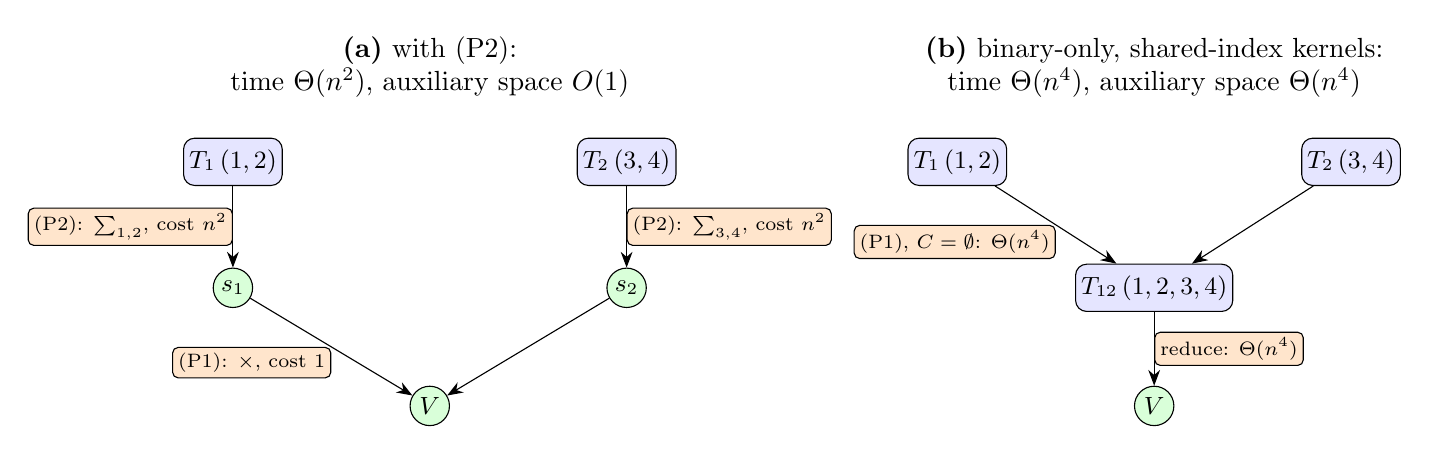
\begin{tikzpicture}[
    tens/.style={draw, fill=blue!10, rounded corners, minimum size=6mm,
                 inner sep=2pt, font=\small},
    scal/.style={draw, fill=green!15, circle, inner sep=1pt,
                 font=\small, minimum size=5mm},
    op/.style={draw, fill=orange!20, rounded corners=2pt, font=\scriptsize,
               inner sep=2pt},
    >={Stealth[length=2mm]},
]
\begin{scope}[xshift=0cm]
  \node[align=center] at (3.3,4.6) {\textbf{(a)} with (P2):\\
        time $\Theta(n^2)$, auxiliary space $O(1)$};
  \node[tens] (T1) at (0.8,3.4) {$T_1$\,$(1,2)$};
  \node[tens] (T2) at (5.8,3.4) {$T_2$\,$(3,4)$};
  \node[scal] (s1) at (0.8,1.8) {$s_1$};
  \node[scal] (s2) at (5.8,1.8) {$s_2$};
  \node[scal] (out)  at (3.3,0.3) {$V$};
  \draw[->] (T1) -- node[op,left] {(P2): $\sum_{1,2}$, cost $n^2$} (s1);
  \draw[->] (T2) -- node[op,right]{(P2): $\sum_{3,4}$, cost $n^2$} (s2);
  \draw[->] (s1) -- node[op,below left]{(P1): $\times$, cost $1$} (out);
  \draw[->] (s2) -- (out);
\end{scope}
\begin{scope}[xshift=9.2cm]
  \node[align=center] at (3.3,4.6) {\textbf{(b)} binary-only, shared-index kernels:\\
        time $\Theta(n^4)$, auxiliary space $\Theta(n^4)$};
  \node[tens] (T1b)  at (0.8,3.4) {$T_1$\,$(1,2)$};
  \node[tens] (T2b)  at (5.8,3.4) {$T_2$\,$(3,4)$};
  \node[tens] (mer) at (3.3,1.8) {$T_{12}$\,$(1,2,3,4)$};
  \node[scal] (outb) at (3.3,0.3) {$V$};
  \draw[->] (T1b) -- node[op,below left] {(P1), $C=\emptyset$: $\Theta(n^4)$} (mer);
  \draw[->] (T2b) -- (mer);
  \draw[->] (mer) -- node[op,right]{reduce: $\Theta(n^4)$} (outb);
\end{scope}
\end{tikzpicture}
\caption{Two contraction trees for $\calA=((1,2),(3,4))$
(Remark~\ref{rem:dcov}).  In (a) the unary reduction collapses each input
to a scalar at cost $\Theta(n^2)$, matching
$n^{\treewidthp{\graphform{\calA}}+1}=n^2$; only $O(1)$ working memory is needed
beyond the inputs.  In (b), without a unary primitive and with
\texttt{tensordot}-style kernels that sum only shared indices, the forced
first step is an outer product that materializes an order-$4$
intermediate: $\Theta(n^4)$ time and working memory.}
\label{fig:dcov-tree}
\end{figure}

% ----------------------------------------------------------------------------
\subsection{Relation to the literature}
% ----------------------------------------------------------------------------

\begin{remark}[Positioning]
\label{rem:lit}
For \emph{closed binary} tensor networks --- every index shared by
exactly two tensors --- Markov and Shi (SIAM J.\ Comput.\ 2008) proved
that the optimal cost of pairwise contraction sequences is governed by
the treewidth of the network's \emph{line graph}; since the line graph of
the tensor-network multigraph is exactly $\graphform{\calA}$ (Section~2
of these notes / new MS Section on the TN duality), Theorem~\ref{thm:main}
specializes to a statement of that type.  The present setting differs in
three ways that the statistical applications force on us: (i)~an index
may occur in three or more tensors (hyperedges), so a binary product may
have to \emph{broadcast} rather than contract; (ii)~an index may occur in
a single tensor and still require summation, so disconnected signatures
such as dCov's need the unary primitive (Remark~\ref{rem:dcov}), a case
outside the closed-network model; (iii)~we track peak memory alongside
time.  Contraction trees of binary networks have also been characterized
via carving width (de Oliveira Oliveira; Dudek, Due\~nas-Osorio and
Vardi), and variable-elimination orderings are classically equivalent to
tree decompositions in the graphical-models and database literatures; to
our knowledge, however, no published statement covers the exact primitive
set (P1)--(P2) of the \Einsum{} libraries with hyperedge signatures,
empty output, disconnected components, and matching time \emph{and}
space bounds.  Practice-side accounts (e.g.\ the \Einsum{} benchmark
literature) note that index-based contraction paths break down precisely
in cases (i)--(ii), but treat this as an engineering matter rather than
proving the equivalence.
\end{remark}

% ============================================================================
\section*{Changelog relative to \texttt{exploration.tex} (for internal review)}
% ============================================================================

\begin{enumerate}
\item \textbf{Lower bound rewritten around an explicit invariant
(Lemma~\ref{lem:invariant}).}  The draft asserted that the co-occurrence
count at elimination time \emph{equals} $\deg_{G^\sigma_{i-1}}$ ``by
Lemma~3 of the main paper applied inductively''.  Two fixes: the relation
is ``$\ge$'' (wasteful broadcasts create extra co-occurrences, which is
harmless), and the MS lemma applies only to index-wise notation
sequences, not to arbitrary pairwise signature lists --- the fill-in
propagation needs its own induction, now spelled out.
\item \textbf{Simultaneous eliminations and tie-breaks.}  A single (P1)
call may eliminate several indices.  Fact~\ref{fact:set-elim}
(order-independent set elimination, path characterization) makes the
partially-eliminated graphs well defined and
Lemma~\ref{lem:per-index} valid for \emph{every} tie-break.
\item \textbf{Upper-bound construction disciplined
(Remark~\ref{rem:early-contraction}).}  The draft's ``contract auxiliary
indices opportunistically'' step could break $\sigma(\Sigma)=\sigma$;
removed.  The draft also both contracted $\sigma[i]$ at the last merge
\emph{and} applied a final unary trace; now exactly one reduction per
step.  Disconnected $\graphform{\calA}$ (leftover scalars per component)
is handled explicitly.
\item \textbf{Space accounting completed.}  The draft counted only the
rolling tensor; the not-yet-consumed step outputs ($\le m$ tensors of
size $\le n^{\wid(\sigma)}$) are now included, with the (always satisfied)
proviso $m \le n$ stated in Assumption~\ref{ass:standing}(iii).
\item \textbf{Prefactor honesty (Remark~\ref{rem:prefactor}).}  The
draft's ``$\asymp |\calA|\, n^{\tw+1}$'' had no matching
$|\calA|$-dependent lower bound; the theorem now states explicit
constants and the fixed-$\calA$ convention.
\item \textbf{dCov remark corrected (Remark~\ref{rem:dcov}).}  With
disjoint signatures the forced first step is a binary merge with
$C=\emptyset$ (an outer product), not a broadcast; under the general
binary primitive the time gap ($n^4$ vs.\ $n^2$) persists, and the space
gap additionally requires the \texttt{tensordot}-style restriction $C
\subseteq B_a \cap B_b$, which is what the libraries' pairwise kernels
implement.  The figure caption now says ``auxiliary space $O(1)$''
rather than ``space $O(1)$''.
\item \textbf{Primitive set simplified.}  Broadcast multiplication (the
draft's (P2)) is the $C=\emptyset$ case of binary contraction; the model
now has two primitives, with the binary one slightly generalized
($C \subseteq B_a \cup B_b$) to match actual binary \Einsum{} calls ---
this strengthens the lower bound and leaves the upper bound valid in the
narrower model (Remark~\ref{rem:naming}).
\end{enumerate}

\end{document}